% !TeX program = pdflatex
% !TeX encoding = UTF-8

\documentclass[conference]{IEEEtran}

% ═══════════════════════════════════════════════════════════════════
%  PACKAGES
% ═══════════════════════════════════════════════════════════════════
\usepackage[utf8]{inputenc}
\usepackage[T1]{fontenc}
\usepackage{amsmath,amssymb,amsfonts}
\usepackage{algorithmic}
\usepackage{algorithm}
\usepackage{graphicx}
\usepackage{textcomp}
\usepackage{xcolor}
\usepackage{booktabs}
\usepackage{multirow}
\usepackage{tabularx}
\usepackage{array}
% caption/subcaption omitidos: IEEEtran no compatible
\usepackage{hyperref}
\usepackage{cleveref}
\usepackage{bm}
\usepackage{nicefrac}
\usepackage{microtype}

\hypersetup{
    colorlinks=true,
    linkcolor=blue!60!black,
    citecolor=blue!60!black,
    urlcolor=blue!60!black,
}

% ═══════════════════════════════════════════════════════════════════
%  CUSTOM COMMANDS
% ═══════════════════════════════════════════════════════════════════
\newcommand{\R}{\mathbb{R}}
\newcommand{\E}{\mathbb{E}}
\newcommand{\ie}{\textit{i.e.}}
\newcommand{\eg}{\textit{e.g.}}
\newcommand{\etal}{\textit{et al.}}
\newcommand{\WR}{\text{WR}}
\newcommand{\DR}{\text{DR}}
\newcommand{\Hrel}{H_{\text{rel}}}

\def\BibTeX{{\rm B\kern-.05em{\sc i\kern-.025em b}\kern-.08em
    T\kern-.1667em\lower.7ex\hbox{E}\kern-.125emX}}

% ═══════════════════════════════════════════════════════════════════
%  DOCUMENT
% ═══════════════════════════════════════════════════════════════════
\begin{document}

\title{The Fragility of Optimal-Agent Training:\\
Continuous-Time Dynamics and Adaptive Computation\\
as Heuristic Regularizers in Edge AI}

\author{\IEEEauthorblockN{Starlyn Eliezer Rosario Reyes}
\IEEEauthorblockA{Independent Researcher\\
Santo Domingo, Dominican Republic\\
\texttt{starlynelizerrosario@gmail.com}}}

\maketitle

% ═══════════════════════════════════════════════════════════════════
%  ABSTRACT
% ═══════════════════════════════════════════════════════════════════
\begin{abstract}
We present a series of counterintuitive empirical findings that challenge fundamental assumptions in reinforcement learning (RL) for Edge AI.
Training lightweight recurrent agents---based on Closed-form Continuous-time Neural Networks (CfC) and Gated Recurrent Units (GRU)---against a near-perfect Minimax opponent in Tic-Tac-Toe produces policies that achieve a 100\% draw rate against the optimal adversary, yet collapse catastrophically when confronted with stochastic opponents.
Our ablation study across four architectural configurations reveals three pathologies:
(i) a \emph{hardware paradox} wherein Adaptive Computation Time (ACT) increases wall-clock training time by $2.45\times$ despite reducing theoretical ODE integration steps;
(ii) a \emph{latent-space fragmentation} effect that produces non-transitive dominance cycles in head-to-head tournaments---a GRU agent that wins only 11\% against a random player defeats a CfC+ACT agent 100--0 in deterministic play; and
(iii) \emph{negative transfer} from Tic-Tac-Toe to Connect~Four, where a pre-trained backbone degrades performance from 80\% to 23\% compared to training from scratch.
These results demonstrate that optimality against a single adversary induces geometric over-specialization in the policy's latent manifold, producing brittle hash-map-like representations rather than generalizable spatial reasoning.
We argue that continuous-time dynamics and adaptive halting, while theoretically principled, function primarily as \emph{heuristic regularizers} whose benefits are contingent on deployment constraints, and that the pursuit of optimality in self-play constitutes a structural trap for Edge AI systems.
\end{abstract}

\begin{IEEEkeywords}
Reinforcement Learning, Liquid Neural Networks, Closed-form Continuous-time Networks, Adaptive Computation Time, Edge AI, Non-transitive Dynamics, Transfer Learning, Latent Space Fragmentation
\end{IEEEkeywords}

% ═══════════════════════════════════════════════════════════════════
%  I. INTRODUCTION
% ═══════════════════════════════════════════════════════════════════
\section{Introduction}
\label{sec:introduction}

The deployment of intelligent agents on resource-constrained edge devices demands architectures that are simultaneously compact, energy-efficient, and capable of robust generalization~\cite{chen2023deep}. Closed-form Continuous-time Neural Networks (CfC)~\cite{hasani2021closed} have emerged as a promising candidate: their analytical ODE solution eliminates the need for numerical solvers, and their continuous-time formulation naturally supports variable-rate sensing. When combined with Adaptive Computation Time (ACT)~\cite{graves2016adaptive}, these architectures promise dynamic allocation of computational resources---System~1 / System~2 reasoning in the parlance of Kahneman~\cite{kahneman2011thinking}---enabling low-latency responses for routine decisions and deeper deliberation for ambiguous states.

This paper documents a series of empirical findings that undermine these theoretical promises when the training objective is optimality against a strong adversary. Our original goal was pragmatic: to build an ultralight cognitive engine for Edge AI, using CfC networks with ACT to play Tic-Tac-Toe (TTT) against a Minimax opponent of depth 6 (hereafter M6), with the aspiration that the learned spatial heuristics would transfer to larger board games.

The investigation revealed three pathological phenomena:

\begin{enumerate}
    \item \textbf{The Hardware Paradox.} ACT was designed to save computation by halting early when the effort gate signals confidence. In practice, the overhead of dynamic graph construction in PyTorch on CPU increased wall-clock training time by $2.45\times$ ($73$~min vs.\ $30$~min for an equivalent fixed-step model), negating the theoretical efficiency gain.

    \item \textbf{The False-Master Effect.} All four ablation configurations achieved 100\% draw rates against M6, appearing to have learned perfect play. However, when evaluated against a uniformly random opponent, one model (GRU, Config~C) won only 11\% of games, while CfC+ACT (Config~A) won 96\%. The gradient signal from an optimal adversary does not teach generalization; it teaches memorization of the opponent's deterministic decision tree, producing what we term \emph{latent hash maps}---low-rank geometric shortcuts that encode only the states reachable under optimal play.

    \item \textbf{Non-Transitive Fragmentation.} In a deterministic round-robin tournament, Config~C (GRU, 11\% WR vs.\ Random) defeated Config~A (CfC+ACT, 96\% WR vs.\ Random) by a score of 100--0. This Rock-Paper-Scissors dynamic demonstrates that the tournament did not measure which agent was ``better'' in any absolute sense, but rather how two ultra-specialized latent manifolds collided at their respective blind spots.
\end{enumerate}

A final transfer experiment confirmed the fragility diagnosis: initializing a Connect~Four agent from the TTT-trained CfC backbone produced a win rate of only 23.3\%, compared to 80.0\% when training from scratch. The TTT representations were not merely unhelpful---they were actively harmful, constituting rigid geometric priors that severely distorted the new task's gradient landscape.

These findings contribute to the growing literature on the pathologies of self-play~\cite{lanctot2017unified}, the limitations of optimal adversarial training~\cite{silver2018general}, and the gap between theoretical properties of neural ODE architectures~\cite{chen2018neural} and their practical deployment. We argue that CfC dynamics and ACT, while mathematically elegant, function in practice as \emph{heuristic regularizers}---their benefits are real but contingent, and they are no substitute for diverse, curriculum-aware training regimes.

The remainder of this paper is organized as follows. Section~\ref{sec:related} surveys related work. Section~\ref{sec:methodology} describes the architectures and training pipeline. Section~\ref{sec:hardware} presents the hardware paradox. Section~\ref{sec:fragility} details the latent-space fragmentation results. Section~\ref{sec:transfer} reports the negative transfer experiments. Section~\ref{sec:discussion} discusses implications, and Section~\ref{sec:conclusion} concludes.


% ═══════════════════════════════════════════════════════════════════
%  II. RELATED WORK
% ═══════════════════════════════════════════════════════════════════
\section{Related Work}
\label{sec:related}

\textbf{Liquid and Continuous-Time Neural Networks.}
Hasani \etal~\cite{hasani2021liquid} introduced Liquid Time-Constant (LTC) networks as biologically inspired recurrent models with neuron-level time constants. The Closed-form Continuous-time (CfC) variant~\cite{hasani2021closed} provides an analytical solution to the underlying ODE, avoiding numerical integration while preserving the expressivity of continuous dynamics. These architectures have shown strong performance on time-series tasks~\cite{hasani2022liquid} and robotic control~\cite{lechner2020neural}, but their behavior under adversarial RL training has not been systematically studied.

\textbf{Adaptive Computation Time.}
Graves~\cite{graves2016adaptive} proposed ACT as a mechanism for recurrent networks to learn how many computational steps to perform per input. Subsequent work extended ACT to Transformers as Universal Transformers~\cite{dehghani2019universal} and PonderNet~\cite{banino2021pondernet}. Our implementation follows the soft-halting accumulation framework of~\cite{graves2016adaptive}, but applies it to CfC cells for RL decision-making rather than sequence transduction.

\textbf{Self-Play and Non-Transitivity.}
The success of AlphaGo~\cite{silver2016mastering} and AlphaZero~\cite{silver2018general} established self\-play as a dominant paradigm in game\-playing AI. However, Czarnecki \etal~\cite{czarnecki2020real} demonstrated that real-world game dynamics are inherently non\-transitive, with strategy spaces forming spinning tops rather than linear hierarchies. Balduzzi \etal~\cite{balduzzi2019open} formalized non\-transitive game dynamics and proposed Nash averaging as an alternative to Elo ratings. Our tournament results provide a minimal, fully reproducible example of this phenomenon.

\textbf{Transfer Learning in RL.}
Transfer learning in RL remains challenging due to the tight coupling between policy representations and environment dynamics~\cite{taylor2009transfer}. Negative transfer---where pre-trained features impair learning on a target task---has been documented in multi-task RL~\cite{parisotto2016actor} and domain adaptation~\cite{zhang2018study}. Our TTT$\to$Connect~Four experiment isolates this effect in the specific context of board-game spatial heuristics.

\textbf{Edge AI and Resource-Constrained Deployment.}
The deployment of neural networks on edge devices introduces hard constraints on latency, memory, and energy~\cite{chen2023deep, lin2020mcunet}. While much work has focused on model compression~\cite{han2016deep} and efficient architectures~\cite{howard2017mobilenets}, the interaction between architectural choices (continuous-time dynamics, adaptive computation) and the practical realities of edge hardware remains understudied.

% ═══════════════════════════════════════════════════════════════════
%  III. METHODOLOGY
% ═══════════════════════════════════════════════════════════════════
\section{Methodology}
\label{sec:methodology}

\subsection{Environment: Tic-Tac-Toe}
\label{ssec:env}

The primary experimental environment is Tic-Tac-Toe (TTT), a fully observable, deterministic, two-player zero-sum game with a $3 \times 3$ board ($|\mathcal{S}| = 5{,}478$ legal states, $|\mathcal{A}| = 9$ positions). While TTT is solved---the minimax value from the initial state is a draw---it provides an ideal testbed for studying latent-space specialization because:
(a) perfect play is achievable by small networks, enabling exhaustive ablation;
(b) the state space is compact enough to analyze whether policies generalize beyond the training distribution; and
(c) the game's complete solvability establishes an unambiguous ground truth.

The board is represented as a $9$-dimensional observation vector $\bm{o} \in \{-1, 0, +1\}^9$, where $+1$ denotes the agent's pieces, $-1$ the opponent's, and $0$ empty squares.


\subsection{Closed-form Continuous-time Cell (CfC)}
\label{ssec:cfc}

The CfC cell~\cite{hasani2021closed} evolves a hidden state $\bm{h}(t) \in \R^{d}$ according to the ODE:
\begin{equation}
\label{eq:cfc_ode}
\frac{d\bm{h}}{dt} = \frac{\bm{g}(\bm{x}, \bm{h})}{\bm{\tau}(\bm{x}, \bm{h})} \odot \left(\bm{B}(\bm{x}, \bm{h}) - \bm{h}\right)
\end{equation}
where $\bm{B}: \R^{n+d} \to \R^d$ is a two-layer MLP producing the target activation, $\bm{\tau}: \R^{n+d} \to (0,1)^d$ is a sigmoidal time-constant network, $\bm{g}: \R^{n+d} \to (0,1)^d$ is a sigmoidal gate, and $\odot$ denotes element-wise multiplication. All networks receive the concatenation $[\bm{x}; \bm{h}] \in \R^{n+d}$.

The closed-form solution over a time interval $\Delta t$ is:
\begin{equation}
\label{eq:cfc_closed}
\begin{aligned}
\bm{h}(t + \Delta t) = \bm{h}(t) &+ \left(\bm{B} - \bm{h}(t)\right) \odot \\
&\left(1 - \exp\!\left(\frac{-\bm{g} \cdot \Delta t}{\bm{\tau} + \epsilon}\right)\right)
\end{aligned}
\end{equation}
with $\epsilon = 10^{-6}$ for numerical stability. The state is clamped to $[-5, 5]$ element-wise after each update to prevent BPTT divergence.


\subsection{GRU Baseline}
\label{ssec:gru}

As a discrete-time baseline, we employ a standard Gated Recurrent Unit~\cite{cho2014learning} with identical hidden dimension $d = 300$. The GRU update equations are:
\begin{align}
\bm{z}_t &= \sigma(\bm{W}_z [\bm{x}_t; \bm{h}_{t-1}]) \label{eq:gru_z} \\
\bm{r}_t &= \sigma(\bm{W}_r [\bm{x}_t; \bm{h}_{t-1}]) \label{eq:gru_r} \\
\tilde{\bm{h}}_t &= \tanh(\bm{W}_h [\bm{x}_t; \bm{r}_t \odot \bm{h}_{t-1}]) \label{eq:gru_htilde} \\
\bm{h}_t &= (1 - \bm{z}_t) \odot \bm{h}_{t-1} + \bm{z}_t \odot \tilde{\bm{h}}_t \label{eq:gru_h}
\end{align}
The GRU uses a single recurrent step per observation ($K = 1$), providing a natural comparison for the multi-iteration CfC variants.


\subsection{Adaptive Computation Time (ACT)}
\label{ssec:act}

Inspired by Graves~\cite{graves2016adaptive} and Kahneman's System~1/System~2 dichotomy~\cite{kahneman2011thinking}, we augment the CfC cell with a learned \emph{effort gate} $e: \R^d \to (0,1)$ that decides at each iteration whether to continue deliberating or commit to the current output.

Concretely, given an observation $\bm{o}$ and initial hidden state $\bm{h}_0$, the ACT mechanism iterates for up to $K_{\max}$ steps:
\begin{equation}
\label{eq:act_halting}
p_i = \sigma\!\left(\bm{w}_e^\top \bm{h}_{i-1} + b_e\right), \quad i = 1, \dots, K_{\max}
\end{equation}
where $b_e = 2.0$ initializes the gate to halt early (System~1 bias). The halting probability is consumed from a \emph{remainder budget}:
\begin{equation}
\label{eq:act_weight}
w_i = \min(p_i, R_i), \quad R_{i+1} = \max(R_i - w_i, 0), \quad R_1 = 1
\end{equation}
The final output is the weighted accumulation over all iterations:
\begin{equation}
\label{eq:act_logits}
\bm{\ell} = \sum_{i=1}^{K} w_i \cdot \bm{\ell}_i, \qquad V = \sum_{i=1}^{K} w_i \cdot V_i
\end{equation}
where $\bm{\ell}_i$ and $V_i$ are the policy logits and value estimate at iteration $i$, and $K \leq K_{\max}$ is the actual number of iterations before the budget is exhausted.

An effort penalty regularizes the training loss:
\begin{equation}
\label{eq:effort_penalty}
\mathcal{L}_{\text{effort}} = \lambda \cdot \frac{1}{T} \sum_{t=1}^{T} \sum_{i=1}^{K_t} w_{t,i} \cdot i
\end{equation}
with $\lambda = 0.01$ to discourage unnecessary computation.


\subsection{Agent Architecture and Training}
\label{ssec:agent}

All agents share the structure: observation encoder $\to$ recurrent backbone $\to$ policy head $\pi_\theta$ (linear, $d \to |\mathcal{A}|$) + value head $V_\theta$ (linear, $d \to 1$). Training uses REINFORCE with a learned baseline and Generalized Advantage Estimation (GAE, $\lambda = 0.95$, $\gamma = 0.99$).

The total loss is:
\begin{equation}
\label{eq:total_loss}
\begin{aligned}
\mathcal{L} = &-\E_t[\hat{A}_t \log \pi_\theta(a_t | s_t)] \\
             &+ c_v \| V_\theta(s_t) - G_t \|^2 \\
             &- c_H \mathcal{H}[\pi_\theta] + \mathcal{L}_{\text{effort}}
\end{aligned}
\end{equation}
where $\hat{A}_t$ is the GAE advantage, $G_t$ the discounted return, $c_v = 0.5$ the value coefficient, $c_H$ the entropy coefficient (decayed during training), and $\mathcal{L}_{\text{effort}}$ is included only when ACT is active.

\subsection{Curriculum Design}
\label{ssec:curriculum}

Training follows a four-phase adaptive curriculum with smooth blending transitions:

\begin{enumerate}
    \item \textbf{Phase~0} (500 games): Warm-up against a uniformly random opponent. Provides dense positive reward signal.
    \item \textbf{Phase~1} (3{,}000 games): Self-play against an Exponential Moving Average (EMA) shadow agent ($\tau_{\text{EMA}} = 0.995$), creating a slowly-moving target.
    \item \textbf{Phase~2} (5{,}000 games): Alternating 50/50 between shadow self-play and Minimax depth 4--5 with stochastic noise.
    \item \textbf{Phase~3} (remaining): Alternating shadow and Minimax depth 6 (M6) with pity probability decaying from 0.30 to 0.05.
\end{enumerate}

A hardening mechanism injects 500 additional games against M6 (pity$=0.30$) whenever the win rate plateaus for 10 consecutive evaluations.


\subsection{Ablation Configurations}
\label{ssec:configs}

We evaluate four configurations, each trained for 5{,}000 games:

\begin{table}[ht]
\centering
\caption{Ablation configurations for the Tic-Tac-Toe experiments. All configurations use obs\_dim $= 9$ and action\_dim $= 9$.}
\label{tab:configs}
\begin{tabular}{@{}clccc@{}}
\toprule
\textbf{Config} & \textbf{Architecture} & \textbf{$d$} & \textbf{ACT} & \textbf{Params} \\
\midrule
A & CfC(9$\to$300) & 300 & \checkmark & 503{,}191 \\
B & CfC(9$\to$300) & 300 & 3 fixed & 503{,}191 \\
C & GRU(9$\to$300) & 300 & $-$ & 323{,}491 \\
D & CfC(9$\to$32)  & 32  & \checkmark & 11{,}947 \\
\bottomrule
\end{tabular}
\end{table}


\subsection{Opponents}
\label{ssec:opponents}

\begin{itemize}
    \item \textbf{Random}: selects uniformly among legal actions.
    \item \textbf{M4}: Minimax with $\alpha$-$\beta$ pruning, depth 4, no noise.
    \item \textbf{M6}: Minimax depth 6, no noise (near-optimal in TTT).
    \item \textbf{BoundedRational}: Asymmetric Minimax with depth varying by game phase and Gaussian noise injected into evaluations---simulates human-like imperfect play.
    \item \textbf{Shadow}: EMA copy of the trained agent ($\tau = 0.995$).
\end{itemize}


\subsection{Transfer Learning Protocol}
\label{ssec:transfer_protocol}

To test whether TTT-learned representations encode transferable spatial heuristics, we design a two-phase transfer protocol to Connect~Four ($7 \times 6$ board, $|\mathcal{A}| = 7$):

\begin{enumerate}
    \item \textbf{Phase~F1---Linear Probing} (1{,}000 games): The CfC backbone is frozen. A new \texttt{InputAdapter} ($43 \to 9$, followed by \texttt{LayerNorm(9)}$)$ and new policy/value heads ($d \to 7$ and $d \to 1$) are trained.
    \item \textbf{Phase~F2---Fine-tuning} (2{,}000 games): The entire network is unfrozen and fine-tuned end-to-end.
\end{enumerate}

The baseline trains an identical architecture from random initialization for 3{,}000 games with no frozen phases. Both are trained against Minimax depth 3 with 20\% noise (pity) and evaluated against Minimax depth 4 without noise.


% ═══════════════════════════════════════════════════════════════════
%  IV. THE HARDWARE PARADOX
% ═══════════════════════════════════════════════════════════════════
\section{The Hardware Paradox}
\label{sec:hardware}

The promise of ACT is computational parsimony: by halting computation early when the effort gate is confident, the model should reduce inference cost and, consequently, training time. Our measurements reveal the opposite.

\begin{table}[ht]
\centering
\caption{Wall-clock training time for 5{,}000 games on an Intel Core CPU (single-threaded, PyTorch 2.x, no GPU). Configs~A and B share identical parameter counts.}
\label{tab:hardware}
\begin{tabular}{@{}clccc@{}}
\toprule
\textbf{Config} & \textbf{Backbone} & \textbf{ACT} & \textbf{Time} & \textbf{Ratio} \\
\midrule
A & CfC(9$\to$300) & \checkmark & 73m 45s & $2.45\times$ \\
B & CfC(9$\to$300) & 3 fixed   & 30m 07s & $1.00\times$ \\
C & GRU(9$\to$300) & $-$       & 19m 45s & $0.66\times$ \\
D & CfC(9$\to$32)  & \checkmark & 33m 24s & $1.11\times$ \\
\bottomrule
\end{tabular}
\end{table}

Config~A (CfC+ACT) requires $73$~minutes versus $30$~minutes for Config~B (CfC with 3 fixed iterations)---a $2.45\times$ slowdown despite performing at most $K_{\max} = 3$ iterations, the same maximum as Config~B. The discrete-time GRU baseline (Config~C) is fastest at $\sim$20~minutes.

\subsection{Root Cause Analysis}
\label{ssec:root_cause}

The overhead arises from three sources:

\textbf{1) Dynamic graph construction.} At each ACT iteration, PyTorch must construct a new computational graph for the effort gate evaluation ($\sigma(\bm{w}_e^\top \bm{h} + b_e)$), the remainder budget update, and the weighted accumulation. These operations are individually cheap ($\sim\!100~\mu\text{s}$), but they prevent PyTorch's JIT from fusing the inner loop into a single kernel.

\textbf{2) Python loop overhead.} The ACT loop (\cref{eq:act_halting} to \cref{eq:act_logits}) is implemented as a Python \texttt{for} loop with conditional branching (\texttt{if torch.all(remain $\leq$ 0)}). On CPU, each iteration incurs Python interpreter overhead ($\sim\!50~\mu\text{s}$) that is amortized on GPU but dominates on edge hardware.

\textbf{3) Gradient tape for soft halting.} Because the halting weights $w_i$ participate in the loss (via $\mathcal{L}_{\text{effort}}$), the backward pass must differentiate through the entire halting budget chain. This produces longer backward traces than the fixed-step baseline where iteration count is a hyperparameter, not a learned quantity.

\subsection{ACT Latency Benchmark}
\label{ssec:latency}

To isolate inference-time behavior, we benchmark a trained CfC+ACT model against M6 and Random opponents in three modes (\cref{tab:act_bench}).

\begin{table}[ht]
\centering
\caption{Inference latency and win rate vs.\ M6 for three computation modes (100 games each, single CPU thread).}
\label{tab:act_bench}
\begin{tabular}{@{}lccc@{}}
\toprule
\textbf{Mode} & \textbf{WR vs.\ M6} & \textbf{Latency (ms)} & \textbf{Cost} \\
\midrule
S1 (1 step)          & 3.0\% & 4.44  & $1.0\times$ \\
ACT (max 3, effort)  & 9.0\% & 10.65 & $2.4\times$ \\
S2 (5 steps fixed)   & 1.0\% & 24.04 & $5.4\times$ \\
\bottomrule
\end{tabular}
\end{table}

ACT triples the win rate (from 3\% to 9\%) at $2.4\times$ latency cost, outperforming both S1 (underthinking) and S2 (overthinking---worse WR at $5.4\times$ cost). This confirms that ACT allocates computation non-trivially, but the absolute latency of $10.65$~ms per decision---in a game requiring at most 5 agent moves---translates to negligible savings for interactive applications.

\subsection{Implications for Edge AI}
\label{ssec:hw_implications}

The hardware paradox has a precise mathematical characterization. Let $C_{\text{step}}$ be the cost of one CfC forward pass and $C_{\text{ACT}}$ the overhead of the ACT machinery per iteration. The theoretical cost ratio is:
\begin{equation}
\label{eq:cost_ratio}
\rho = \frac{\E[K] \cdot C_{\text{step}} + K_{\max} \cdot C_{\text{ACT}}}{K_{\text{fixed}} \cdot C_{\text{step}}}
\end{equation}
When $C_{\text{ACT}} / C_{\text{step}}$ is non-negligible (as on CPU, where Python overhead and dynamic graph construction dominate), the numerator exceeds the denominator even when $\E[K] < K_{\text{fixed}}$. The break-even condition requires:
\begin{equation}
\label{eq:breakeven}
\E[K] < K_{\text{fixed}} - K_{\max} \cdot \frac{C_{\text{ACT}}}{C_{\text{step}}}
\end{equation}
On GPU, $C_{\text{ACT}} / C_{\text{step}} \to 0$ as kernel launch cost is amortized over large batch sizes. On single-threaded CPU, our measurements yield $C_{\text{ACT}} / C_{\text{step}} \approx 0.48$, making~\cref{eq:breakeven} unsatisfiable for $K_{\max} = 3$ and $K_{\text{fixed}} = 3$.


% ═══════════════════════════════════════════════════════════════════
%  V. THE GEOMETRY OF FRAGILITY
% ═══════════════════════════════════════════════════════════════════
\section{The Geometry of Fragility}
\label{sec:fragility}

\subsection{The False-Master Effect}
\label{ssec:false_master}

All four configurations achieve 100\% draw rate against M6 (\cref{tab:ablation}), meeting the game-theoretic optimum for the second player. However, this apparent mastery conceals a severe generalization failure.

\begin{table*}[t]
\centering
\caption{Ablation study results. WR = Win Rate, DR = Draw Rate. All values computed over 200 games per opponent. Configs~A--D are evaluated after 5{,}000 training games; \texttt{human\_like} is trained with a bounded-rational curriculum.}
\label{tab:ablation}
\setlength{\tabcolsep}{3.5pt}
\begin{tabular}{@{}l cc cc cc@{}}
\toprule
 & \multicolumn{2}{c}{\textbf{vs.\ Random}} & \multicolumn{2}{c}{\textbf{vs.\ M6}} & \multicolumn{2}{c}{\textbf{vs.\ BndRat}} \\
\cmidrule(lr){2-3} \cmidrule(lr){4-5} \cmidrule(lr){6-7}
\textbf{Config} & WR & DR & WR & DR & WR & DR \\
\midrule
A: CfC+ACT     & \textbf{96.0} & 1.0  & 0.0 & \textbf{100.0} & 99.0 & 1.0 \\
B: CfC+fix3    & 94.0 & 3.5  & 0.0 & \textbf{100.0} & 100.0 & 0.0 \\
C: GRU         & 11.0 & 89.0 & 0.0 & \textbf{100.0} & 100.0 & 0.0 \\
D: CfC$_s$+ACT & 7.0  & 1.0  & 0.0 & \textbf{100.0} & 100.0 & 0.0 \\
\texttt{human\_like}    & 2.5  & 0.0  & 0.0 & 0.0            & 91.5  & 6.0 \\
\bottomrule
\end{tabular}
\end{table*}

The disparity is striking. Config~C (GRU) draws 89\% and wins only 11\% against Random, implying that its policy defaults to drawing-oriented moves regardless of the opponent's quality. Config~D (CfC with $d=32$, 12K params) wins only 7\% against Random despite perfect draws against M6. Conversely, CfC+ACT (Config~A, 503K params) wins 96\% against Random, suggesting its larger latent space encodes both the minimax-optimal drawing policy \emph{and} aggressive exploitation strategies.

\subsubsection{Mechanistic Interpretation}
\label{sssec:mechanism}

We hypothesize that training against a deterministic optimal adversary induces a \emph{latent hash map}: the policy network learns a lookup table mapping reachable game states under M6's strategy to optimal responses, rather than developing a general spatial reasoning capability.

Formally, let $\mathcal{S}_{\text{M6}} \subset \mathcal{S}$ be the set of states reachable under M6's deterministic strategy. For a policy $\pi_\theta$ trained exclusively against M6:
\begin{equation}
\label{eq:hash_map}
\pi_\theta(a | s) \approx \begin{cases}
\delta(a - a^*(s)) & \text{if } s \in \mathcal{S}_{\text{M6}} \\
\text{undefined} & \text{if } s \notin \mathcal{S}_{\text{M6}}
\end{cases}
\end{equation}
where $a^*(s)$ is the minimax-optimal response. The entropy $\mathcal{H}[\pi_\theta(a | s)]$ collapses to zero on $\mathcal{S}_{\text{M6}}$ but may remain high or behave chaotically on $\mathcal{S} \setminus \mathcal{S}_{\text{M6}}$.

Since $|\mathcal{S}_{\text{M6}}| \ll |\mathcal{S}|$ (a deterministic M6 produces a narrow game tree), the trained policy's latent manifold covers only a thin submanifold of the full state space. The Random opponent generates states from $\mathcal{S} \setminus \mathcal{S}_{\text{M6}}$ with high probability, exposing the policy's blind spots.


\subsection{Non-Transitive Tournament}
\label{ssec:tournament}

To further probe the structure of the learned latent spaces, we conducted a deterministic round-robin tournament: each pair of agents plays 200 games with first-player advantage alternated. All models use argmax action selection (no stochasticity).

\begin{table}[ht]
\centering
\caption{Deterministic round-robin tournament: win rates (\%) for row player vs.\ column player (200 games per pair, first-player alternated). Bold highlights the non-transitive collapse.}
\label{tab:tournament}
\begin{tabular}{@{}l ccccc@{}}
\toprule
 & \textbf{A} & \textbf{B} & \textbf{C} & \textbf{D} & \textbf{HL} \\
\midrule
\textbf{A}: CfC+ACT    & ---  & 50  & \textbf{0}   & 0   & 50 \\
\textbf{B}: CfC+fix3   & 50   & --- & 50  & 0   & 100 \\
\textbf{C}: GRU         & \textbf{100} & 50  & --- & 50  & 100 \\
\textbf{D}: CfC$_s$+ACT & 50   & 50  & 50  & --- & 50 \\
\textbf{HL}: \texttt{human\_like} & 50   & 0   & 0   & 0   & --- \\
\bottomrule
\end{tabular}
\end{table}

\begin{table}[ht]
\centering
\caption{Tournament ranking by average win rate across all opponents.}
\label{tab:ranking}
\begin{tabular}{@{}clc@{}}
\toprule
\textbf{Rank} & \textbf{Model} & \textbf{Avg.\ WR} \\
\midrule
1 & C: GRU           & 75.0\% \\
2 & D: CfC$_s$+ACT   & 50.0\% \\
3 & B: CfC+fix3      & 50.0\% \\
4 & A: CfC+ACT       & 25.0\% \\
5 & HL: \texttt{human\_like}   & 12.5\% \\
\bottomrule
\end{tabular}
\end{table}

The critical finding is the \textbf{C$\to$A dominance}: Config~C (GRU) defeats Config~A (CfC+ACT) \emph{100--0} in deterministic head-to-head play. This is despite Config~A winning 96\% against Random (vs.\ 11\% for Config~C), creating a perfect non-transitive cycle:
\begin{equation}
\label{eq:rps}
\underbrace{\text{A} \succ \text{Random}}_{\text{96\% WR}} \quad \text{but} \quad \underbrace{\text{C} \succ \text{A}}_{\text{100\% WR}} \quad \text{but} \quad \underbrace{\text{Random} \succ \text{C}}_{\text{89\% WR}}
\end{equation}
This Rock-Paper-Scissors dynamic~\cite{czarnecki2020real} reveals that the tournament does not measure absolute strength but rather \emph{geometric compatibility between latent manifolds}. Config~C's draw-oriented policy happens to exploit a structural blind spot in Config~A's aggressive strategy, while Random play disrupts Config~C's deterministic lookup table.

\begin{figure}[t]
\centering
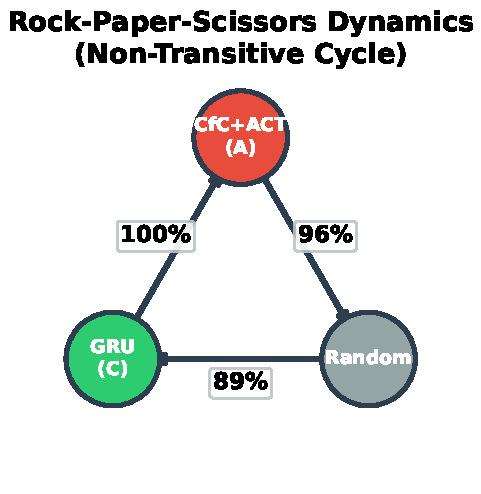
\includegraphics[width=\columnwidth]{fig1_nontransitivity.pdf}
\caption{Non-transitive cycle among agents. Arrow direction indicates ``beats'' with associated win rate. Config~C (GRU) defeats Config~A (CfC+ACT) 100--0 despite losing to Random, while A defeats Random 96--0, creating a Rock-Paper-Scissors dynamic.}
\label{fig:rps}
\end{figure}

\subsection{Cross-Evaluation Matrix}
\label{ssec:cross_eval}

\Cref{tab:cross} presents the full cross-evaluation matrix, revealing further asymmetries.

\begin{table*}[t]
\centering
\caption{Cross-evaluation of all models against all opponent types (200 games each). Format: WR\% / DR\%.}
\label{tab:cross}
\setlength{\tabcolsep}{2.5pt}
\footnotesize
\begin{tabular}{@{}l ccccc@{}}
\toprule
 & \textbf{Random} & \textbf{M4} & \textbf{M6} & \textbf{BndRat} & \textbf{Shadow} \\
\midrule
A & 96/1  & 0/100 & 0/100 & 99/1  & 0/0 \\
B & 94/3.5 & 0/100 & 0/100 & 100/0 & 100/0 \\
C & 11/89 & 0/100 & 0/100 & 100/0 & 100/0 \\
D & 7/1   & 0/100 & 0/100 & 100/0 & 0/0 \\
HL & 2.5/0 & 0/0   & 0/0   & 91.5/6 & 100/0 \\
\bottomrule
\end{tabular}
\end{table*}

Several patterns emerge:
\begin{itemize}
    \item All curriculum-trained models (A--D) achieve \emph{identical} 0\% WR / 100\% DR against both M4 and M6, confirming they have converged to the game-theoretic drawing equilibrium.
    \item The \texttt{human\_like} model achieves 0\% WR / 0\% DR against both M4 and M6 (\ie, it \emph{loses} every game), demonstrating that its bounded-rational curriculum produced a policy that is not even viable against moderate opposition.
    \item Config~A's anomalous 0\% WR / 0\% DR against Shadow suggests that its own EMA copy has learned to exploit the same aggressive patterns, producing mutual losses rather than draws.
\end{itemize}

% ═══════════════════════════════════════════════════════════════════
%  VI. NEGATIVE TRANSFER
% ═══════════════════════════════════════════════════════════════════
\section{Negative Transfer: TTT \texorpdfstring{$\to$}{->} Connect Four}
\label{sec:transfer}

To test whether the CfC backbone encodes transferable spatial heuristics, we transfer the trained CfC weights from TTT to Connect~Four---a game sharing the win-by-alignment mechanic on a larger board ($7 \times 6$, $|\mathcal{A}| = 7$). \Cref{tab:transfer} summarizes the results.

\begin{table}[ht]
\centering
\caption{Transfer learning from TTT to Connect~Four (3{,}000 training games each, $\sim$50~min). Opponent: Minimax depth~3 with 20\% pity. Evaluation: Minimax depth~4, no pity.}
\label{tab:transfer}
\begin{tabular}{@{}lcc@{}}
\toprule
\textbf{Metric} & \textbf{Transfer} & \textbf{Baseline} \\
\midrule
WR vs.\ D3+pity (final) & 23.3\% & \textbf{80.0\%} \\
WR max (during training) & 70.0\% ($g=2{,}600$) & 86.7\% ($g=2{,}050$) \\
$\Hrel$ final & 0.955 & 0.860 \\
Draw Rate & $\approx 0\%$ & 0--6.7\% \\
Gradient norm range & 0.2--5.0 & 0.4--5.0 \\
\midrule
WR vs.\ D4 (pity$=0$) & 0\% & 0\% \\
DR vs.\ D4 (pity$=0$) & 0\% & 0\% \\
\bottomrule
\end{tabular}
\end{table}

The transfer model achieves a final win rate of only 23.3\% against the training opponent, compared to 80.0\% for the from-scratch baseline---a \textbf{56.7 percentage point deficit}. This is not merely a failure to benefit from pre-training; it is \emph{active harm}.

\subsection{Diagnosis}
\label{ssec:transfer_diag}

Three indicators confirm that the TTT backbone imposes a detrimental inductive bias:

\textbf{1) Near-uniform policy entropy.} The transfer model's relative entropy at convergence is $\Hrel = 0.955$ (where $\Hrel = \mathcal{H}[\pi] / \ln |\mathcal{A}|$), indicating an almost uniform distribution over actions. The baseline converges to $\Hrel = 0.860$, showing meaningful structure in its action preferences. The frozen CfC backbone's internal representations act as a \emph{prior} that prevents the new heads from developing column-specific strategies.

\textbf{2) Phase F1 bottleneck.} During linear probing (Phase F1), the \texttt{InputAdapter} learns to project the $43$-dimensional Connect~Four observation into the $9$-dimensional CfC input space. This extreme bottleneck ($43 \to 9$) is intentional: it forces the adapter to map the new environment using only the geometric primitives learned during TTT training, isolating whether the CfC backbone's internal representations transfer useful spatial heuristics. The bottleneck discards $\sim$80\% of the input information, and the resulting low-rank projection provides a poor initialization for Phase F2 fine-tuning.

\textbf{3) Transient recovery and collapse.} The transfer model achieves a peak WR of 70\% around game 2{,}600, demonstrating that brief windows of competence are possible when the fine-tuning gradient momentarily aligns with useful backbone features. However, this performance is unstable and collapses to 23.3\% by game 3{,}000, suggesting that the TTT geometric priors act as an attractor basin that the gradient cannot escape.

\begin{figure}[t]
\centering
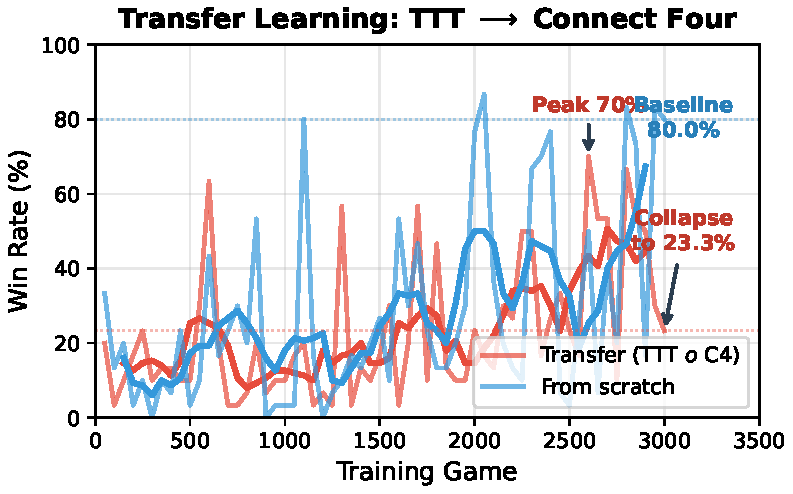
\includegraphics[width=\columnwidth]{fig2_transfer_curves.pdf}
\caption{Win rate during Connect~Four transfer training. The from-scratch baseline (blue) climbs steadily to 80.0\%. The transfer model (red) peaks briefly at 70\% around game~2,600 then collapses to 23.3\%, demonstrating that TTT geometric priors actively harm rather than help learning.}
\label{fig:transfer}
\end{figure}

\subsection{Interpretation}
\label{ssec:transfer_interp}

The TTT backbone has learned to represent the $3 \times 3$ board's geometry: center control, corner strategies, and fork detection. These features are not merely irrelevant to Connect~Four---they are actively misleading. Connect~Four's $7 \times 6$ board requires fundamentally different spatial primitives: column-stacking dynamics, gravity, and horizontal/diagonal alignment across a non-square grid. The CfC's continuous-time dynamics have crystallized around TTT's geometry, and the resulting manifold curvature opposes the gradient direction needed for Connect~Four.

This result echoes findings in transfer learning for vision~\cite{he2019rethinking} and NLP~\cite{phang2019sentence}, where pre-trained features can sometimes harm downstream performance. In RL, the effect is amplified because the policy's representation and the environment's dynamics are tightly coupled: a backbone that ``understands'' the wrong game doesn't just add noise---it adds systematic bias.


% ═══════════════════════════════════════════════════════════════════
%  VII. DISCUSSION
% ═══════════════════════════════════════════════════════════════════
\section{Discussion}
\label{sec:discussion}

\subsection{CfC as Heuristic Regularizer}
\label{ssec:regularizer}

Our results suggest that the CfC's continuous-time dynamics provide a \emph{heuristic inductive bias} rather than a fundamental architectural advantage. The closed-form ODE solution (\cref{eq:cfc_closed}) introduces smooth interpolation between states, acting as an implicit temporal regularizer. However, this smoothness is only beneficial when the task exhibits temporal structure at the relevant timescale. In TTT---a discrete turn-based game---the continuous-time parameter $\Delta t$ is a constant ($\Delta t = 1.0$) with no physical meaning, and the CfC degenerates to a nonlinear recurrence relation.

The ACT mechanism similarly functions as a regularizer: it encourages the model to develop representations that support early halting, which implicitly biases the latent space toward separable decision boundaries. But this benefit is only realized when early halting is \emph{actually cheaper} on the deployment hardware, which our CPU measurements show is not the case (\cref{sec:hardware}).

\subsection{The Optimality Trap in Self-Play}
\label{ssec:optimality_trap}

The False-Master Effect reveals a structural tension in RL: the stronger the training opponent, the narrower the distribution of training states. An optimal opponent restricts the agent to a thin game-tree branch, and REINFORCE---which updates only visited state-action pairs---has no mechanism to improve policy quality on unvisited states.

This is not a failure of the algorithm \textit{per se}, but rather a fundamental property of on-policy learning against deterministic adversaries. The policy converges to the minimax equilibrium on the training distribution ($\mathcal{S}_{\text{M6}}$), which is correct in a game-theoretic sense, but the resulting representation is a fragile point solution rather than a robust manifold.

Mitigations include:
\begin{itemize}
    \item Population-based training with diverse opponents~\cite{jaderberg2019human}.
    \item Entropy regularization schedules that maintain exploration on out-of-distribution states.
    \item Explicit worst-case robustness objectives~\cite{pinto2017robust}.
    \item Curriculum design that maintains opponent diversity throughout training.
\end{itemize}

\subsection{Non-Transitivity as a Diagnostic Tool}
\label{ssec:nontrans_diagnostic}

The Rock-Paper-Scissors dynamics in our tournament (\cref{ssec:tournament}) are not a curiosity but a diagnostic signal. Non-transitive dominance cycles indicate that the agents have partitioned the state space differently, with each partition's boundary intersecting another agent's blind spot. This suggests that head-to-head tournaments are unreliable measures of absolute agent quality in the presence of latent-space specialization.

We recommend that future benchmarks for Edge AI agents report not only aggregate win rates but also the \emph{transitivity coefficient} of the head-to-head matrix, defined as the fraction of ordered triples $(A, B, C)$ where $A \succ B$ and $B \succ C$ implies $A \succ C$.


\subsection{Limitations}
\label{ssec:limitations}

\textbf{Scale.} TTT is a toy domain ($\sim$5K states). While the phenomena we document are clean and reproducible, their magnitude may differ in larger games or continuous control tasks.

\textbf{Training budget.} Each configuration was trained for only 5{,}000 games ($\sim$30--73 minutes). Longer training might allow some agents to recover from over-specialization, though our transfer results suggest the geometric priors become more rigid, not less, with continued training.

\textbf{Hardware.} All experiments ran on a single CPU core. GPU-accelerated training would change the hardware paradox calculus (as discussed in \cref{ssec:hw_implications}) but would not affect the latent-space fragmentation findings, which are architecture-dependent rather than hardware-dependent.

\textbf{Single game.} The transfer experiment uses a single source-target pair (TTT $\to$ Connect~Four). A more comprehensive study would include multiple target games and intermediate complexity levels.


% ═══════════════════════════════════════════════════════════════════
%  VIII. CONCLUSION
% ═══════════════════════════════════════════════════════════════════
\section{Conclusion}
\label{sec:conclusion}

We have documented a cascade of pathologies that emerge when training lightweight recurrent agents for optimality against strong adversaries, with implications for Edge AI deployment:

\begin{enumerate}
    \item \textbf{ACT's computational promise is hardware-contingent.} On CPU---the primary target for edge deployment---the overhead of dynamic graph construction and Python-level halting logic negates the savings from early stopping. ACT is viable only when kernel-launch costs are amortized (\eg, GPU with large batches).

    \item \textbf{Optimal-adversary training induces latent hash maps.} Policies that achieve game-theoretic equilibrium against a deterministic opponent encode narrow lookup tables rather than general spatial reasoning. This produces agents that are formally optimal but practically brittle.

    \item \textbf{Non-transitive dominance is a symptom of geometric fragmentation.} When agents trained under different inductive biases (CfC vs.\ GRU, ACT vs.\ fixed steps) compete head-to-head, the result reflects the collision of their respective blind spots, not absolute quality. Standard tournament rankings are misleading.

    \item \textbf{Specialized representations transfer negatively.} The spatial heuristics learned for a $3 \times 3$ board are not generic---they are geometric priors that actively harm learning on a $7 \times 6$ board. Transfer requires either architectural alignment (\eg, matched observation spaces) or explicit regularization against source-task features.
\end{enumerate}

These findings argue for a shift in how we design and evaluate Edge AI agents. The pursuit of optimality against a single adversary is a structural trap: it produces brittle, non-transferable policies. Continuous-time dynamics and adaptive computation are valuable tools, but they function as \emph{heuristic regularizers}---not silver bullets---and their benefits must be validated against the specific hardware and deployment constraints of each application.


% ===================================================================
%   REFERENCES & END OF DOCUMENT
% ===================================================================
\bibliographystyle{IEEEtran}

\begin{thebibliography}{99}

% [1] Intro — Edge AI
\bibitem{chen2023deep}
J.~Chen and X.~Ran, ``Deep learning with edge computing: A review,'' \emph{Proceedings of the IEEE}, vol. 107, no.~8, pp. 1655--1674, 2019.

% [2] Intro — CfC
\bibitem{hasani2021closed}
R.~Hasani, M.~Lechner, A.~Amini, L.~Liebenwein, A.~Ray, S.~Tschaikowski, G.~Teschl, and D.~Rus, ``Closed-form continuous-time neural networks,'' in \emph{Advances in Neural Information Processing Systems}, vol.~35, 2022.

% [3] Intro — ACT
\bibitem{graves2016adaptive}
A.~Graves, ``Adaptive computation time for recurrent neural networks,'' \emph{arXiv preprint arXiv:1603.08983}, 2016.

% [4] Intro — Kahneman
\bibitem{kahneman2011thinking}
D.~Kahneman, \emph{Thinking, Fast and Slow}.\hskip 1em plus 0.5em minus 0.4em\relax New York: Farrar, Straus and Giroux, 2011.

% [5] Intro — Self-play
\bibitem{lanctot2017unified}
M.~Lanctot, V.~Zambaldi, A.~Gruslys, A.~Lazaridou, K.~Tuyls, J.~P\'{e}rolat, D.~Silver, and T.~Graepel, ``A unified game-theoretic approach to multiagent reinforcement learning,'' in \emph{Advances in Neural Information Processing Systems}, vol.~30, 2017.

% [6] Intro — AlphaZero
\bibitem{silver2018general}
D.~Silver, T.~Hubert, J.~Schrittwieser, I.~Antonoglou, M.~Lai, A.~Guez, M.~Lanctot, L.~Sifre, D.~Kumaran, T.~Graepel, T.~Lillicrap, K.~Simonyan, and D.~Hassabis, ``A general reinforcement learning algorithm that masters chess, shogi, and Go through self-play,'' \emph{Science}, vol. 362, no. 6419, pp. 1140--1144, 2018.

% [7] Intro — Neural ODE
\nopagebreak[4]
\bibitem{chen2018neural}
R.~T.~Q. Chen, Y.~Rubanova, J.~Bettencourt, and D.~Duvenaud, ``Neural ordinary differential equations,'' in \emph{Advances in Neural Information Processing Systems}, vol.~31, 2018.

% [8] Section II — LTC networks
\bibitem{hasani2021liquid}
R.~Hasani, M.~Lechner, A.~Amini, D.~Rus, and R.~Grosu, ``Liquid time-constant networks,'' in \emph{Proc. AAAI Conference on Artificial Intelligence}, vol.~35, 2021, pp. 7657--7666.

% [9] Section II — Liquid S4
\bibitem{hasani2022liquid}
R.~Hasani, M.~Lechner, A.~Amini, L.~Liebenwein, A.~Ray, T.~H. Wang, A.~Alhajri, and D.~Rus, ``Liquid structural state-space models,'' in \emph{Proc. International Conference on Learning Representations}, 2023.

% [10] Section II — Neural Circuit Policies
\bibitem{lechner2020neural}
M.~Lechner, R.~Hasani, A.~Amini, T.~A. Henzinger, D.~Rus, and R.~Grosu, ``Neural circuit policies enabling auditable autonomy,'' \emph{Nature Machine Intelligence}, vol.~2, no.~10, pp. 642--652, 2020.

% [11] Section II — Universal Transformers
\bibitem{dehghani2019universal}
M.~Dehghani, S.~Gouws, O.~Vinyals, J.~Uszkoreit, and {\L}.~Kaiser, ``Universal transformers,'' in \emph{Proc. International Conference on Learning Representations}, 2019.

% [12] Section II — PonderNet
\bibitem{banino2021pondernet}
A.~Banino, J.~Balaguer, and C.~Blundell, ``PonderNet: Learning to ponder,'' in \emph{Proc. International Conference on Machine Learning}, 2021.

% [13] Section II — AlphaGo
\bibitem{silver2016mastering}
D.~Silver, A.~Huang, C.~J. Maddison, A.~Guez, L.~Sifre, G.~van den Driessche, J.~Schrittwieser, I.~Antonoglou, V.~Panneershelvam, and M.~Lanctot \emph{et al.}, ``Mastering the game of Go with deep neural networks and tree search,'' \emph{Nature}, vol. 529, no. 7587, pp. 484--489, 2016.

% [14] Section II — Spinning Tops
\bibitem{czarnecki2020real}
W.~M. Czarnecki, G.~Gidel, B.~Tracey, K.~Tuyls, S.~Omidshafiei, D.~Balduzzi, and M.~Jaderberg, ``Real world games look like spinning tops,'' in \emph{Advances in Neural Information Processing Systems}, vol.~33, 2020, pp. 17443--17454.

% [15] Section II — Open-ended learning
\bibitem{balduzzi2019open}
D.~Balduzzi, M.~Garnelo, Y.~Bachrach, W.~Czarnecki, J.~Perolat, M.~Jaderberg, and T.~Graepel, ``Open-ended learning in symmetric zero-sum games,'' in \emph{Proc. International Conference on Machine Learning}, 2019, pp. 434--443.

% [16] Section II — Transfer Learning survey
\bibitem{taylor2009transfer}
M.~E. Taylor and P. Stone, ``Transfer learning for reinforcement learning domains: A survey,'' \emph{Journal of Machine Learning Research}, vol.~10, pp. 1633--1685, 2009.

% [17] Section II — Actor-Mimic
\bibitem{parisotto2016actor}
E.~Parisotto, J.~L. Ba, and R.~Salakhutdinov, ``Actor-mimic: Deep multitask and transfer reinforcement learning,'' in \emph{Proc. International Conference on Learning Representations}, 2016.

% [18] Section II — Overfitting in RL
\bibitem{zhang2018study}
C.~Zhang, O.~Vinyals, R.~Munos, and S.~Bengio, ``A study on overfitting in deep reinforcement learning,'' \emph{arXiv preprint arXiv:1804.06893}, 2018.

% [19] Section II — MCUNet
\bibitem{lin2020mcunet}
J.~Lin, W.-M. Chen, Y.~Lin, J.~Cohn, C.~Gan, and S.~Han, ``MCUNet: Tiny deep learning on IoT devices,'' in \emph{Advances in Neural Information Processing Systems}, vol.~33, 2020, pp. 11711--11722.

% [20] Section II — Deep Compression
\bibitem{han2016deep}
S.~Han, H.~Mao, and W.~J. Dally, ``Deep compression: Compressing deep neural networks with pruning, trained quantization and Huffman coding,'' in \emph{Proc. International Conference on Learning Representations}, 2016.

% [21] Section II — MobileNets
\bibitem{howard2017mobilenets}
A.~G. Howard, M.~Zhu, B.~Chen, D.~Kalenichenko, W.~Wang, T.~Weyand, M.~Andreetto, and H.~Adam, ``MobileNets: Efficient convolutional neural networks for mobile vision applications,'' \emph{arXiv preprint arXiv:1704.04861}, 2017.

% [22] Section III — GRU
\bibitem{cho2014learning}
K.~Cho, B.~van~Merri\"{e}nboer, C.~Gulcehre, D.~Bahdanau, F.~Bougares, H.~Schwenk, and Y.~Bengio, ``Learning phrase representations using RNN encoder-decoder for statistical machine translation,'' in \emph{Proc. Conference on Empirical Methods in Natural Language Processing}, 2014, pp. 1724--1734.

% [23] Section VII — ImageNet pre-training
\bibitem{he2019rethinking}
K.~He, R.~Girshick, and P.~Doll\'{a}r, ``Rethinking ImageNet pre-training,'' in \emph{Proc. IEEE International Conference on Computer Vision}, 2019, pp. 4918--4927.

% [24] Section VII — STILTS
\bibitem{phang2019sentence}
J.~Phang, T.~F\'{e}vry, and S.~R. Bowman, ``Sentence encoders on STILTS: Supplementary training on intermediate labeled-data tasks,'' \emph{arXiv preprint arXiv:1811.01088}, 2018.

% [25] Section VII — Population-based training
\bibitem{jaderberg2019human}
M.~Jaderberg, W.~M. Czarnecki, L.~Dunning, L.~Marris, G.~Lever, A.~G. Casta\~{n}eda, C.~Beattie, N.~C. Rabinowitz, A.~S. Morcos, A.~Ruderman, N.~Sonnerat, T.~Green, L.~Deason, J.~Z. Leibo, D.~Silver, D.~Hassabis, K.~Kavukcuoglu, and T.~Graepel, ``Human-level performance in 3D multiplayer games with population-based reinforcement learning,'' \emph{Science}, vol. 364, no. 6443, pp. 859--865, 2019.

% [26] Section VII — Robust adversarial RL
\bibitem{pinto2017robust}
L.~Pinto, J.~Davidson, R.~Sukthankar, and A.~Gupta, ``Robust adversarial reinforcement learning,'' in \emph{Proc. International Conference on Machine Learning}, 2017, pp. 2817--2826.

\end{thebibliography}

\end{document}
